\lecture{9}{24. Februar 2025}{Failure Mechanisms, pt. 1: Static Loading and Fracture}

\section{Fundamentals of Fracture}
\begin{dis}[Cite two situations in which the possibility of failure is part of the design of a compononent or product]
  Lots of products are made in such a way that them failing is central to their function. Examples include:
  \begin{itemize}
    \item Electrical fuses
    \item Pull tabs on soda cans
    \item The metal fencing between driveways in opposite directions on highways
    \item Many sprinkler systems inside homes
    \item and much more
  \end{itemize}
\end{dis}
Before delwing into a discussion about fracturing it is very important to have some basic definitions in place.
\begin{definition}[Fracture]
  A \textit{fracture} is the separation of a body into two or more pieces in response to a stress. A fracture can either be \textit{cohesive}, if the fracture happens within the material itself or \textit{adhesive} if it happens at the intersection between two materials or phases.
\end{definition}
In general there are two types of fractures. These are split into
\begin{definition}[Ductile fractures]
  A \textit{ductile fracture} is characterized by rather slow crack propagation and ductile fracturing is accompanied by significant plastic deformation -- It \textit{fails with warning} so to say. For examples of this please refer to \textbf{\Cref{fig:f9_1,fig:f9_2,fig:f9_3}}.
\end{definition}
\begin{figure} [ht]
  \centering
  \caption{Fracture profiles for 3 different materials ranging from \textit{Very Ductile} to \textit{Brittle}}
  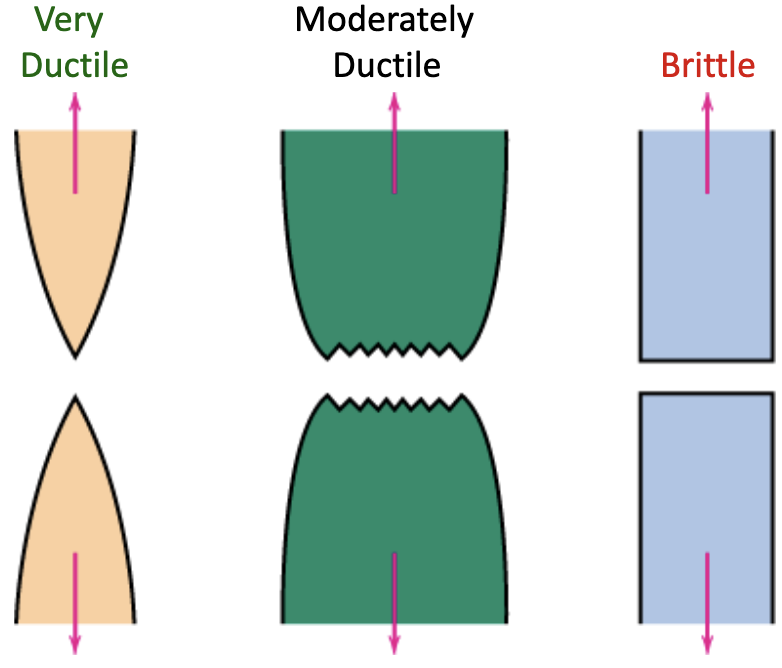
\includegraphics[width=0.25\linewidth]{./figures/f9_1.png}
  \label{fig:f9_1}
\end{figure}
\begin{definition}[Brittle fractures]
  A \textit{brittle fracture} is characterized by very rapid crack propagation -- often in the order of the speed of sound. Brittle fracturing happens with little or no plastic deformation at all -- It ``fails without warning'' so to say. For examples of this please refer to \textbf{\Cref{fig:f9_1,fig:f9_2,fig:f9_3}}.
\end{definition}
In general ductile fracturing is more desirable than brittle fracturing but it of course depends on the application.
\begin{figure}[ht]
  \centering
  \begin{minipage}{0.58\linewidth}
    \centering
    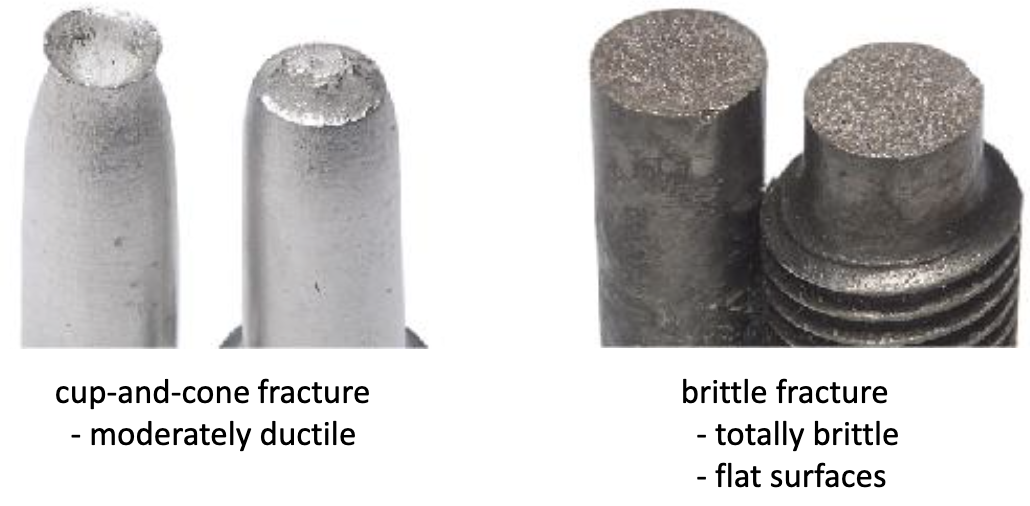
\includegraphics[width=\linewidth]{./figures/f9_2.png}
    \caption{Fracture surfaces for a \textit{moderately ductile} and a \textit{totally brittle} material.}
    \label{fig:f9_2}
  \end{minipage}
  \hfill
  \begin{minipage}{0.38\linewidth}
    \centering
    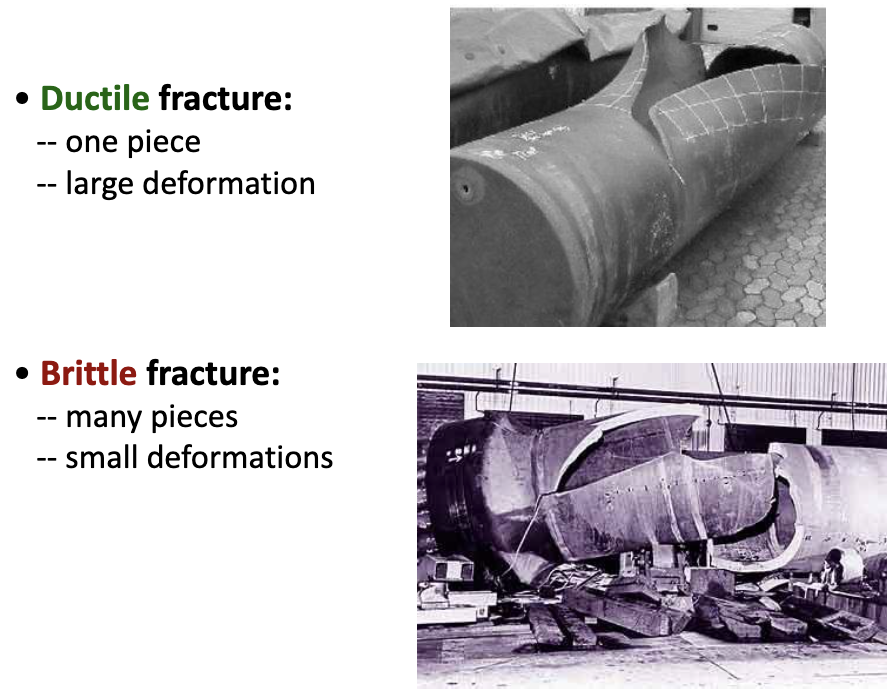
\includegraphics[width=\linewidth]{./figures/f9_3.png}
    \caption{\textit{Ductile} and \textit{brittle} fracturing in pipes.}
    \label{fig:f9_3}
  \end{minipage}
\end{figure}


The \textit{cup-and-cone} fracture as seen on \textbf{\autoref{fig:f9_2}} is a rather characteristic fracture type for moderately ductile materials. In general the process of a moderately ductile fracture are
\begin{enumerate}
  \item \textbf{Necking:} When a moderately ductile material is exposed to a strong tensile stress it will start to \textit{neck}, meaning it will start to get smaller (plastically deform) around the part of the sample that is later going to break.
  \item \textbf{Void nucleation:} Within the necked region, microscopic voids will start to form. These voids often originate at imperfections, such as inclusions or second-phase particles, which act as stress concentrators. To see this please refer to \textbf{\autoref{fig:f9_4}}. 
  \item \textbf{Void growth and coalescence:} As deformation continues, these nucleated voids grow in size. Eventually, adjacent voids merge (coalesce) forming microcracks within the material.
  \item \textbf{Crack propagation and Fracture:} Once a critical level of void coalescence is reached, a crack begins to propagate rapidly through the material, leading to seperation into two or more pieces.
\end{enumerate}
All of these stages are shown graphically on \textbf{\autoref{fig:f9_4}}.
\begin{figure} [ht]
  \centering
  \caption{The stages of fracture of a moderately ductile material}
  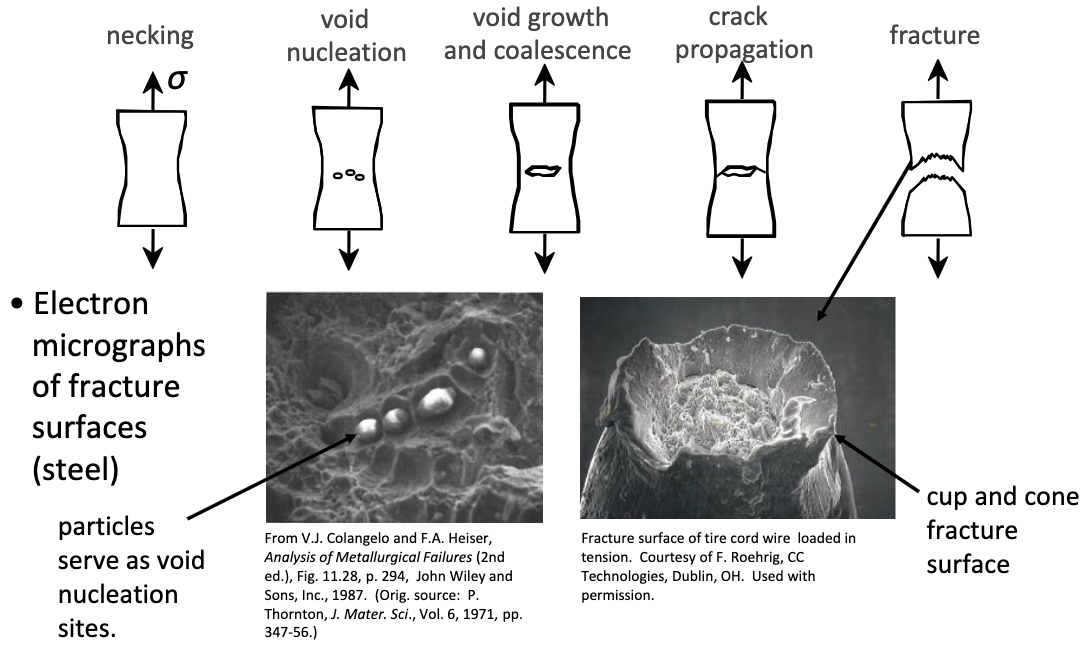
\includegraphics[width=0.5\linewidth]{./figures/f9_4.png}
  \label{fig:f9_4}
\end{figure}

\section{Failure Mechanics}
Both the Titanic and many of the so-called Liberty ships built in the second world war failed in a brittle manner. This stands in sharp contrast to the ductility of steel one had found in tension tests in laboratories. It was for a long time a mystery why so many ships were suddenly becoming brittle rather than ductile and it took quite a while until we figured out that steel becomes brittle under the so-called \textit{ductile-brittle transition temperature}. This real-life example highlights the importance of understanding fracture mechanics and gaining an understanding about how the use-case of a material might affect its properties. In short, the measured fracture strength of materials is lower than that predicted by theory. This is due to inherent flaws (in the form of microscopic cracks) in the material. These cracks act as stress-amplifiers as an applied stress will become many times bigger in magnitude around these cracks. This is shown on \textbf{\autoref{fig:f9_5}}.

\begin{figure} [ht]
  \centering
  \caption{Concentration of stress around flaws}
  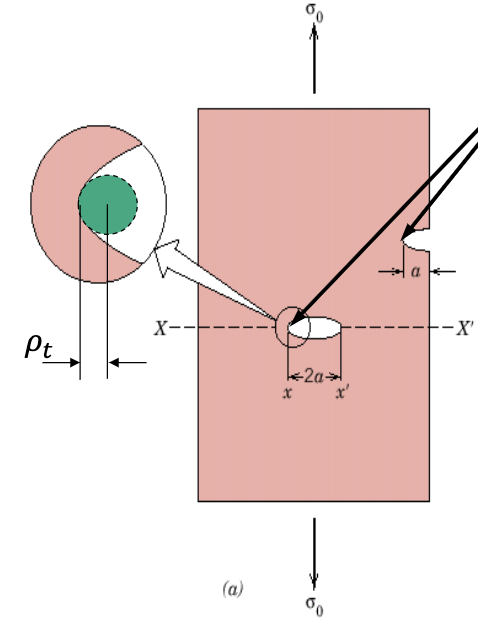
\includegraphics[width=0.25\linewidth]{./figures/f9_5.png}
  \label{fig:f9_5}
\end{figure}

\subsection{Stress concentration} \label{sec:strcon}
We are actually able to form a mathematical expression for the amount of stress measured exactly at the tip of the flaw ($\sigma_m$) just using the dimensions shown in \textbf{\autoref{fig:f9_5}}. This is
\[ 
\sigma_m = 2\sigma_0 \sqrt{\frac{a}{\rho_t}}
\]
where $\sigma_0$ is the applied bulk stress, $\rho_t$ is the radius of curvature of the tip of the flaw and $a$ is the half length of the elliptical (or crack-like) flaw. Thus even a small crack with a very sharp tip can amplify the stress many times. Analog to this we can define the \textit{stress concentration factor} $K_t$, as the ratio of the peak stress at the crack/hole boundary $\sigma_m$ to the nominal far-field stress $\sigma_0$:
\[ 
K_t = \frac{\sigma_m}{\sigma_0}
.\]
In real life the amplified stress is not only concentrated at the tip or edge of the defect but but most of the additional stress will be seen in an area very close to the defect as seen on \textbf{\autoref{fig:f9_6}}. The amplification of stress at edges of defects is also the reason that samples with sharp corners tend to fail more easily than samples with filleted edges. The effect of material dimensions and the corresponding change in strength is shown on \textbf{\autoref{fig:f9_7}}.

\begin{figure}[ht]
  \centering
  \begin{minipage}{0.33\linewidth}
    \centering
    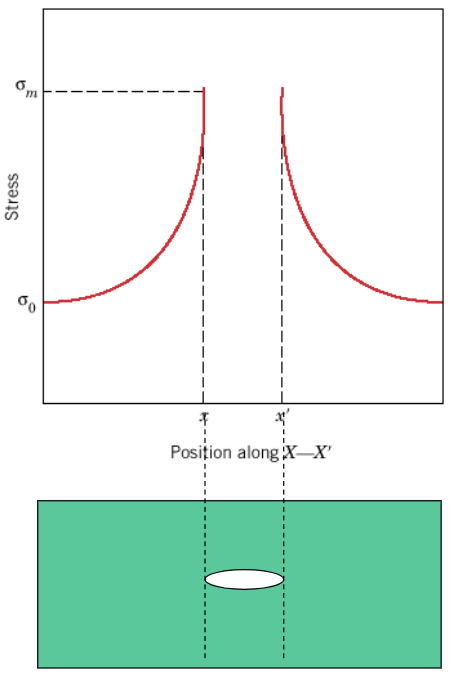
\includegraphics[width=\linewidth]{./figures/f9_6.png}
    \caption{Increase in stress concentration close to the edges of defects}
    \label{fig:f9_6}
  \end{minipage}
  \hfill
  \begin{minipage}{0.65\linewidth}
    \centering
    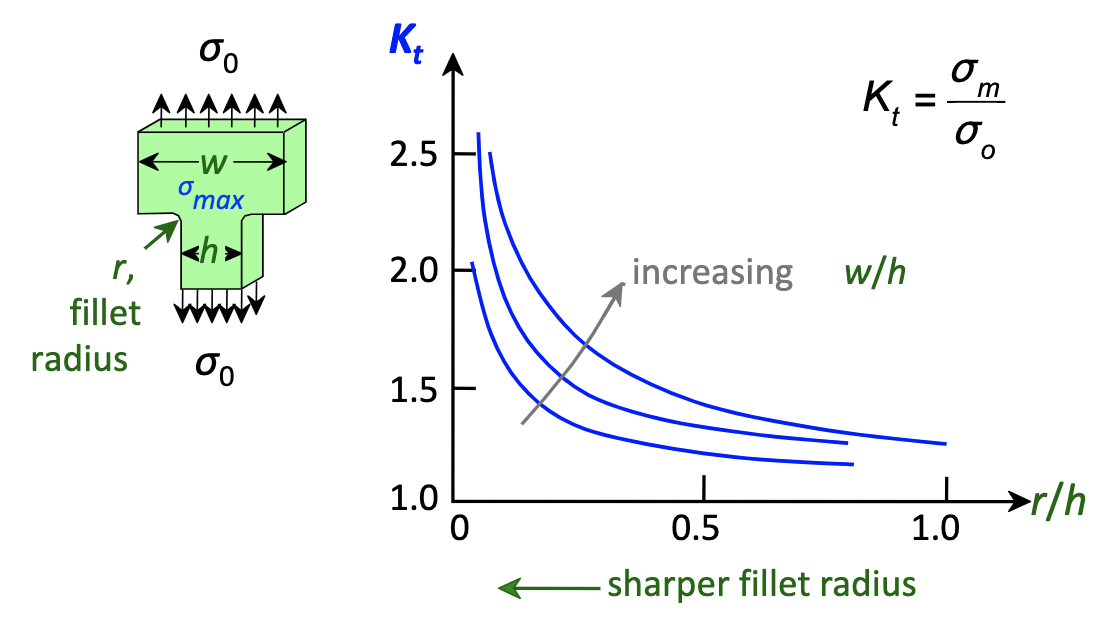
\includegraphics[width=\linewidth]{./figures/f9_7.png}
    \caption{Implication of dimensions on fracture properties}
    \label{fig:f9_7}
  \end{minipage}
\end{figure}

\subsection{Crack propagation}
As explained in \textbf{\autoref{sec:strcon}} an applied external stress is concentrated and amplified at the edges of cracks, defects or other imperfections. Sharper edges of these imperfections leads to more amplification of the applied stress and if the edges are too sharp or the bulk stress is too high the cracks will start to expand and propagate. Ductile materials will experience this effect to a lesser degree than an otherwise similar but ductile material as the ductile material will deform around the edges of the imperfections in such a way that it minimizes the stress (in this case the edge of the crack will deform and become more blunt).

Assuming you are working with a brittle material it is possible to determine the critical stress for crack propagation $\sigma_c$ as
\[
  \sigma_c = \sqrt{\frac{2E \gamma_s}{\pi a}}
\]
Where $E$ is Young's modulus, $\gamma_s$ is the specific surface energy and $a$ is the half length of an internal crack. For brittle materials the specific surface energy $\gamma_s$ should be replaced with $\gamma_s + \gamma_p$ where $\gamma_p$ is the plastic deformation energy. It is important to note that materials have numerous crack with different lengths and orientations. Crack propagation (and fracture) occurs when $\sigma_m > \sigma_c$ for the crack with the lowest $\sigma_c$ -- this also means that the largest and most stresset cracks will grow first.


\section{Fracture Toughness}
The \textit{fracture toughness} of a material is a measure of its resistance to brittle fracture when a crack is present. The fracture toughness is defined as
\[ 
K_{Ic} = Y \sigma_c \sqrt{\pi a}
.\]
Where $Y$ is a dimensionless parameter often written as $f(a / W)$ which accounts for the specimen's geometry and the crack's position, $\sigma_c$ is the critical stress for crack propagation and $a$ is the crack length.  The fracture toughness $K_c$ is essentially the critical stress intensity beyond which a crack will rapidly propagate. 

\subsection{Fracture modes}
Fractures can be split loosely into 3 categories:
\begin{enumerate}
  \item \textbf{Opening/Tensile Mode:} The crack faces are pulled apart directly away from each other. This is the most common (and often most severe) mode, where the crack ``opens up'' under tensile stress. This is the mode labelled $(a)$ on \textbf{\autoref{fig:f9_8}}.
  \item \textbf{Sliding/In-Plane Shear Mode:} The load is applied parallel to the crack front, causing the two crack faces to slide relative to each other in the plane of the crack. This is the mode labelled $(b)$ in \textbf{\autoref{fig:f9_8}}.
  \item \textbf{Tearing/Anti-Plane Shear Mode:} The load is, again, parallel to the crack front, but in a direction out of the crack plane. You can think of one crack face ``twisting'' relative to the other. This is the mode labelled $(c)$ in \textbf{\autoref{fig:f9_8}}.
\end{enumerate}
\begin{figure} [ht]
  \centering
  \caption{The three main fracture modes}
  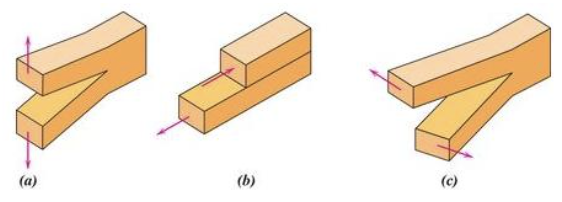
\includegraphics[width=0.5\linewidth]{./figures/f9_8.png}
  \label{fig:f9_8}
\end{figure}

\section{Design Implications}
The above considerations can be summarised in the so-called \textit{crack growth condition}:
\[ 
K_{Ic} < Y \sigma_c \sqrt{\pi a}
.\]
This can then be used in some different ways. For example
\begin{itemize}
  \item If you are given the materials fracture toughness $K_{Ic}$ and the flaw size $a$ you are able to find the maximum design (critical) stress as
    \[ 
    \sigma_c = \frac{K_{Ic}}{Y \sqrt{\pi a}}
    .\]
  \item If you know the fracture toughness of the material $K_{Ic}$ and the applied stress $\sigma$ you can find the maximum allowable flaw size as
    \[ 
    a_c = \frac{1}{\pi} \left( \frac{K_{Ic}}{Y \sigma} \right)^2
    .\]
\end{itemize}
